\documentclass[12pt, a4paper]{report}

\usepackage[czech]{babel}
\usepackage[utf8]{inputenc}
%\usepackage[cp1250]{inputenc}
\usepackage[IL2]{fontenc}
\usepackage{anyfontsize}
\usepackage{graphicx}
\usepackage{float}
\usepackage{color}

\title{Manuál aplikace MediTab}
\author{David Pivovar}

%%%%%%%%%%%%%%%%%%%%%%%%%%%%%%%%%%%%%%%%%%%%%%%%%%%%%%%%%%%
%%%%%Makra%%%%%%%%%%%%%%%%%%%%%%%%%%%%%%%%%%%%%%%%%%%%%%%%%

% Tato makra přesvědčují mírně ošklivým trikem LaTeX, aby hlavičky kapitol
% sázel příčetněji a nevynechával nad nimi spoustu místa. Směle ignorujte.
\makeatletter
\def\@makechapterhead#1{
  {\parindent \z@ \raggedright \normalfont
   \Huge\bfseries \thechapter. #1
   \par\nobreak
   \vskip 20\p@
}}
\def\@makeschapterhead#1{
  {\parindent \z@ \raggedright \normalfont
   \Huge\bfseries #1
   \par\nobreak
   \vskip 20\p@
}}
\makeatother

% Toto makro definuje kapitolu, která není očíslovaná, ale je uvedena v obsahu.
\def\chapwithtoc#1{
\chapter*{#1}
\addcontentsline{toc}{chapter}{#1}
}



%%%%%%%%%%%%%%%%%%%%%%%%%%%%%%%%%%%%%%%%%%%%%%%%%%%%%%%%%%%
%%%%%Zacatek dokumentu%%%%%%%%%%%%%%%%%%%%%%%%%%%%%%%%%%%%%

\begin{document}

%%%%%%%%%%%%%%%%%%%%%%%%%%%%%%%%%%%%%%%%%%%%%%%%%%%%%%%%%%%
%%%%%Titulni strana%%%%%%%%%%%%%%%%%%%%%%%%%%%%%%%%%%%%%%%%
\begin{titlepage}

\begin{center}

\vspace*{50pt}
	
	{\fontsize{36}{0} \textbf{
		{\color{red}MediTab}
	}}
	
	\vfill
	
	{\fontsize{28}{0} \textbf{
		Manuál
	}}
	
	\vfill
	\vfill
	
	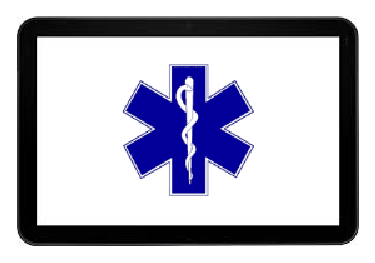
\includegraphics[width=0.7\textwidth]{img/logo_wide.eps}

\end{center}

\vspace{110pt}

\begin{flushleft}

	{\fontsize{20}{0} \selectfont
		David Pivovar\\[5pt]
		%Daniel Švarc
		\hfill
		Verze 1.0
	}
	
\end{flushleft}

\end{titlepage}


\tableofcontents

%%%%%%%%%%%%%%%%%%%%%%%%%%%%%%%%%%%%%%%%%%%%%%%%%%%%%%%%%%%
%%%%%Kapitoly%%%%%%%%%%%%%%%%%%%%%%%%%%%%%%%%%%%%%%%%%%%%%%

\chapter*{Úvod}
\addcontentsline{toc}{chapter}{Úvod}

Předmětem této práce je vytvořit grafické uživatelské rozhraní tabletové aplikace pro jednotku intenzivní péče ve Fakultní nemocnici v Plzni. Tato aplikace je určena především pro zdravotní sestry. Na nemocničním pokoji bude k dispozici tablet s aplikací, kde zdravotní sestra bude mít k dispozici aktuální data o pacientech a bude do aplikace zanamenávat své provedené úkony.

Aplikace nahradí tištěnou formu medikačních záznamů a záznamů o pacientech. Umožní tak okamžitý přístup k datům v databázi a zefektivní proces přenosu a ukládání nových aktuálních dat. Aplikace zefektivní práci jak zdravotních sester, tak i lékařů. Každý provedený úkon zdravotní sestrou se okamžitě promítne do databáze a lékař ho uvidí na svém PC. Díky propojení dat s databází se předejde ručnímu přepisování, při kterém se zvyšuje chybovost.

Cílem je vytvořit jednoduché a intuitivní uživatelské rozhraní, které se podobá zavedeným postupům ve FN Plzeň. Vzorem pro vývoj tabletové aplikace je desktopová aplikace WinMedicalc vyvíjená plzeňskou firmou Medicalc software s.r.o. ve spolupráci se SIS FN Plzeň\footnote{Správa informačního systému (IT oddělení nemocnice)}.

Tabletovou aplikaci pro jednotku intenzivní péče jsem nazval pracovním názvem \emph{MediTab}.

V první časti této práce je popsáno prostředí jednotky intenzivní péče nemocnice a aplikace WinMedicalc, části, které jsou společné s vyvíjenou aplikací (kapitola \ref{ch:fn}). Druhá část se zabývá požadavky na vyvíjenou aplikaci (kapitola \ref{ch:specifikace}) a jejím návrhem (kapitola \ref{ch:navrh}). V poslední části je popsána implementace uživatelského rozhraní (kapitola \ref{ch:implementace}) a průběh testování aplikace (kapitola \ref{ch:test}).
\chapter{Manuál}

%%%%%%%%%%%%%%%%%%%%%%%%%%%%%%%%%%%%%%%%%%%%%%%%%%%%%%%%%%%


\end{document}
